\section{The Model}
\label{sec:model}

This section describes the Chronotypic Market Ecology (CME) model in full. The model is a computer simulation, so every rule below is something the computer actually executes, step by step, many times. We describe each piece in words first, then give the formula.

\subsection{Investors and their trading horizons}

The simulated market has $n=80$ investors. Each investor $i$ has a \emph{trading horizon} $\tau_i$, measured in trading days, between 1 and 2{,}000 days. We draw horizons from four investor types designed to mimic the real mix of institutional money in 2023. Table~\ref{tab:types} lists them.

\begin{table}[htbp]
\centering
\caption{The four investor types. A horizon is drawn from a log-normal distribution with the stated parameters (on a log scale), keeping only draws inside the stated range.}
\label{tab:types}
\begin{tabular}{lrrrr}
\toprule
Type & Horizon range (days) & Log-normal $(\mu,\sigma)$ & Share of assets & Investors\\
\midrule
High-frequency trader & 1 to 20 & (0.5, 0.6) & 15\% & 12\\
Hedge fund & 15 to 120 & (2.8, 0.7) & 25\% & 20\\
Mutual fund & 60 to 400 & (4.2, 0.6) & 40\% & 32\\
Pension fund & 400 to 2{,}000 & (6.0, 0.8) & 20\% & 16\\
\bottomrule
\end{tabular}
\end{table}

A log-normal distribution is natural here because horizons span several orders of magnitude, and the difference between a 5-day and a 10-day horizon matters as much as the difference between 500 and 1{,}000 days. Working on a log scale respects that.

\subsection{How investors demand shares and how the price moves}

Every period, each investor decides how much to buy or sell. We write their demand $d_i(t)$ at time $t$. It has three parts:
\begin{equation}
d_i(t) \;=\; \underbrace{\bar\alpha\,\frac{F_t-\bar p_i(t)}{p_t}}_{\text{value investing}}
\;+\; \underbrace{\bar\beta\, m_i(t)}_{\text{trend following}}
\;+\; \underbrace{\varepsilon_i(t)}_{\text{noise}} .
\label{eq:demand}
\end{equation}

\begin{itemize}[leftmargin=*]
\item \textbf{Value investing.} $F_t$ is the true fundamental value of the asset. It moves randomly: $F_t = F_{t-1}\exp(\varepsilon^F_t)$ with $\varepsilon^F_t$ normal with standard deviation $0.010$. $\bar p_i(t)$ is investor $i$'s own average of recent prices, over the last $\tau_i$ days. If this average is below the fundamental value, the investor thinks the asset is cheap and buys. The weight is $\bar\alpha = 0.30$.
\item \textbf{Trend following.} $m_i(t)=\ln\big(p(t)/p(t-\tau_i)\big)$ is how much the price has risen over the investor's own horizon. A rising price encourages buying. The weight is $\bar\beta=0.20$. Notice that this is where an investor's horizon matters: a short-horizon investor reacts to the last few days, a long-horizon investor to the last few years.
\item \textbf{Noise.} $\varepsilon_i(t)$ is random demand unrelated to the first two terms. It is normal with standard deviation $\sigma_i^{\mathrm{eff}}$, defined next.
\end{itemize}

A single market maker sets the next price in proportion to the total net demand:
\begin{equation}
p(t+1) \;=\; p(t) + \lambda \sum_{i=1}^{n} d_i(t), \qquad \lambda = 0.008 .
\label{eq:price}
\end{equation}
So if buyers outnumber sellers the price rises, and the parameter $\lambda$ says by how much. All trades pass through this market maker. The network described below governs how investors share \emph{information and beliefs}, not who trades with whom directly. This is a simplification: it ignores the order book and the fact that a pension fund would rarely be the direct counterparty of a high-frequency trader.

\subsection{Cross-horizon friction}

Why might horizon similarity matter for volatility? The model's answer is \emph{friction}: an investor who deals with counterparties on very different time scales has a harder time reading signals, so their demand is noisier. We write the noise level of investor $i$ as
\begin{equation}
\sigma^{\mathrm{eff}}_i \;=\; \sigma_0\big(1+\gamma\,\bar d_\tau(i)\big), \qquad \sigma_0 = 1,\ \gamma = 0.20,
\label{eq:sigeff}
\end{equation}
where $\bar d_\tau(i)$ is the average distance, on the log scale, between investor $i$'s horizon and the horizons of the investors linked to them. When $i$'s neighbours are close in horizon, $\bar d_\tau$ is small and noise is low. When neighbours are far away in horizon, noise is higher. Setting $\gamma=0$ switches the friction off, which we use as a test below. This channel is the \emph{only} way that clustering reduces volatility in the model, and it will matter again in Section~\ref{sec:tension}.

\subsection{The horizon network and horizon clustering}

Investors are linked in a directed network. The probability that investor $i$ links to investor $j$ depends on how close their horizons are:
\begin{equation}
P(i\to j) \;\propto\; \exp\!\big(-\kappa_h\,\big|\ln(\tau_i+1)-\ln(\tau_j+1)\big|\big).
\label{eq:network}
\end{equation}
The symbol $\propto$ means the probabilities are rescaled so that each investor's link probabilities sum to one. The parameter $\kappa_h\ge 0$ is the \emph{horizon clustering strength}. When $\kappa_h=0$ the exponent is zero for everyone, every investor is equally likely to link to every other, and the network is random. As $\kappa_h$ rises, links between investors with very different horizons become rare.

\begin{example}[Three investors]
Take three simulated investors P, Q, R with horizons 5, 20 and 400 days. On the log scale ($\ln(\tau+1)$) their positions are 1.79, 3.04 and 5.99. The distances are $|P-Q|=1.25$ and $|P-R|=4.20$.

If $\kappa_h=0$, P is equally likely to link to Q or R (50\% each).

If $\kappa_h=1$, the unnormalised weights are $e^{-1.25}=0.286$ for Q and $e^{-4.20}=0.015$ for R. Rescaling to sum to one, P links to Q with probability $0.286/(0.286+0.015)\approx 95\%$ and to R with probability about 5\%.

Higher $\kappa_h$ pushes this further, so that investors almost exclusively link to others with similar horizons.
\end{example}

Figure~\ref{fig:tikz} sketches the effect. With no clustering, links cross the whole horizon range. With strong clustering, links stay among near neighbours and the network breaks into horizon-based cliques.

\begin{figure}[htbp]
\centering
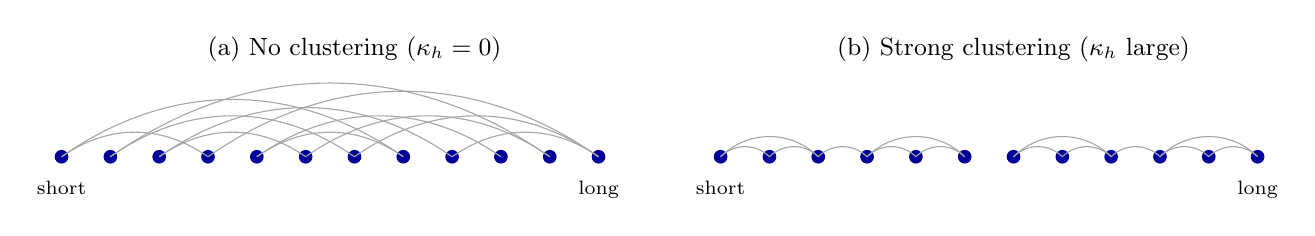
\begin{tikzpicture}[scale=0.62,>=stealth]
% left panel: no clustering
\begin{scope}
\node at (6,2.2) {\small (a) No clustering ($\kappa_h=0$)};
\foreach \i in {0,...,11} {\fill[blue!60!black] (\i,0) circle (0.14);}
\foreach \a/\b in {0/7,1/10,2/5,3/11,4/9,6/11,0/3,2/8,5/10,1/6,4/7,8/11} {\draw[gray!70] (\a,0) to[bend left=35] (\b,0);}
\node[below] at (0,-0.3) {\scriptsize short};\node[below] at (11,-0.3) {\scriptsize long};
\end{scope}
\begin{scope}[xshift=13.5cm]
\node at (6,2.2) {\small (b) Strong clustering ($\kappa_h$ large)};
\foreach \i in {0,...,11} {\fill[blue!60!black] (\i,0) circle (0.14);}
\foreach \a/\b in {0/1,1/2,0/2,3/4,4/5,3/5,6/7,7/8,6/8,9/10,10/11,9/11,2/3,8/9} {\draw[gray!70] (\a,0) to[bend left=45] (\b,0);}
\node[below] at (0,-0.3) {\scriptsize short};\node[below] at (11,-0.3) {\scriptsize long};
\end{scope}
\end{tikzpicture}
\caption{Illustration (not simulation output). Twelve investors arranged from short to long horizon. Without clustering, links cross the horizon range. With strong clustering, links join near neighbours, producing horizon-based cliques.}
\label{fig:tikz}
\end{figure}

\subsection{Horizon adaptation}

Investors are influenced by those they deal with. Every cycle, each investor moves their horizon a fraction $\eta=0.06$ of the way toward the average horizon of their linked neighbours:
\begin{equation}
\tau_i \;\leftarrow\; (1-\eta)\,\tau_i + \eta\,\bar\tau_{\mathcal N(i)} .
\label{eq:adapt}
\end{equation}
For example, a high-frequency trader with $\tau=5$ whose only neighbour has $\tau=1000$ moves to $5+0.06\times(1000-5)\approx 65$ days. In the full network, where neighbours average a few hundred days, the typical shift is more modest (about 15 days per cycle). The economic idea is a simple form of social learning: an investor who spends time among long-horizon counterparties comes to take on their way of looking at the market. Repeated over many cycles, adaptation pulls horizons together and so reduces the diversity of horizons. We call this the \emph{echo-chamber} effect.

\subsection{Three diagnostic measures}

We summarise the state of the simulated market with three numbers.

\paragraph{Horizon diversity (Temporal Diversity Index, TDI).} How spread out are investors' horizons? We split the log-horizon scale from $\ln 1$ to $\ln 2000$ into $K=16$ equal-width bins, compute the fraction $f_k$ of investors in each bin, and take the Shannon entropy,
\begin{equation}
\mathrm{TDI} \;=\; -\sum_{k=1}^{K} f_k\,\ln f_k .
\label{eq:tdi}
\end{equation}
Entropy is a standard measure of spread. If everyone sits in a single bin, TDI is zero. If investors are spread evenly over all bins, TDI is at its maximum. In the simulation the full range is available, so the largest possible value is $\ln 16\approx 2.77$. In the real-data analysis of Section~\ref{sec:data}, horizons are limited to at least 5 days, so the three lowest bins are always empty and the largest possible value is $\ln 13\approx 2.565$.

\begin{example}[Toy calculation of horizon diversity]
Suppose, to keep arithmetic small, that we use only five bins and that 20\%, 30\%, 30\%, 10\% and 10\% of investors fall in them. Then
\[
\mathrm{TDI} = -\big[0.2\ln 0.2 + 2\times 0.3\ln 0.3 + 2\times 0.1\ln 0.1\big]
= 0.322 + 0.722 + 0.461 = 1.505 .
\]
The maximum possible with five bins is $\ln 5 = 1.609$ (an even split), so this market is fairly diverse. If everyone were in one bin the value would be $0$.
\end{example}

\paragraph{Belief fragmentation (Temporal Market Fragmentation Index, TMFI).} Do investors in different horizon groups hold different beliefs about the price? We sort investors into four groups by horizon (quartiles of $\ln(\tau+1)$). Each investor forms a noisy view of the price, $\hat p_i = p\,(1+\sigma_{\mathrm{obs}}\xi_i)$ with $\sigma_{\mathrm{obs}}=0.008$ and $\xi_i$ random. We average these views within each group, and TMFI is the standard deviation of the four group averages divided by their mean:
\begin{equation}
\mathrm{TMFI}(t) \;=\; \frac{\mathrm{std}\big(\{\bar p^{(c)}(t)\}_{c=1}^{4}\big)}{\mathrm{mean}\big(\{\bar p^{(c)}(t)\}_{c=1}^{4}\big)} .
\label{eq:tmfi}
\end{equation}
Before averaging, each investor's view is blended with those of their network neighbours, with a weight that rises with the network's overall connectedness (measured by its Fiedler value, $\lambda_2$, which is a standard measure of how well connected a network is). A high TMFI means groups disagree about the price. A low TMFI means beliefs are aligned.

\paragraph{Temporal liquidity (TL).} How smoothly does price information move across horizons? We define
\begin{equation}
\mathrm{TL}(t)\;=\;\frac{1}{\sigma_r(t)\,|\mathrm{ACF}_1(t)|},
\label{eq:tl}
\end{equation}
where $\sigma_r$ is the volatility of returns and $\mathrm{ACF}_1$ is the first-order autocorrelation of returns (how strongly one period's return predicts the next). The idea is that a liquid market has both low volatility and little predictable pattern in returns. We will see in Section~\ref{sec:tl} that because volatility sits inside this measure, any comparison of TL with a volatility index is partly mechanical.

\subsection{A note on stability}

A natural worry for any simulation is whether prices simply blow up. A standard linear analysis gives a sufficient condition for stability in terms of the network: $\lambda_2>\bar\beta/\bar\alpha$. In our calibration $\bar\beta/\bar\alpha = 0.667$ while the simulated Fiedler value is about $0.655$, so the condition fails in 27 of 30 runs. This does \emph{not} mean prices explode; the condition is sufficient, not necessary. In the simulation prices stay bounded because the value-investing term in Eq.~\eqref{eq:demand} acts as a nonlinear restoring force that the linear analysis does not capture. We therefore treat the Fiedler value as a diagnostic of network connectivity, not as the governing stability criterion.

One further check concerns the simplest disturbance, a uniform shift in the price. A fractional price shift $\delta$ changes every investor's trend signal by $\delta$, and so changes next period's price by $\lambda n\bar\beta\,\delta$. Relative to the price level of 100, the one-step gain is $\lambda n \bar\beta/100 = 0.008\times 80\times 0.20/100\approx 1.3\times 10^{-3}$, far below one. A shock of this kind therefore dies out by a factor of about a thousand each period, so this mode is not a concern.
